% Implement Chapter Continued
\section{Boot Process}\index{Boot Process}
% \begin{lstlisting}[language=bash]
%   $ aws s3 cp whirlpool-cf-template.yml s3://whirlpool-cf-templates/
% 
%   $ aws cloudformation create-stack \
%   --stack-name whirlpool-crawler \
%   --template-body <x.yml> \
%   --profile whirlpool \
% 
%   $ scp prod-docker-compose.yml whirlpool-crawler-1:~/
% 
%   $ docker-compose -f prod-docker-compose.yml up -d
% 
%   $ aws cloudformation delete-stack --stack-name whirlpool-crawler
% \end{lstlisting}

A fresh installation of whirlpool crawler comprising of multiple services begins by first packaging
production code for each service as docker image. The below code snippet shows \texttt{Dockerfile}
of \texttt{whirpool-fetch} component. Lines 1, 28, and 31 show \texttt{dev} and \texttt{prod} target images  get derived from \texttt{base} image. The specialized image produced differ by configurations, evironment
variables, etc.

\inputminted[
fontfamily=tt,
baselinestretch=1.2,
fontsize=\footnotesize,
linenos,
numbersep=5pt,
tabsize=2,
frame=single]{yaml}{../../whirlpool/crawler/whirlpool-fetch/Dockerfile}

\pagebreak

\noindent
The below command packages production docker image from base layer, skipping dev layer.

\begin{lstlisting}[language=bash]
  $ docker build -t whirlpool-fetch-prod:latest --target whirlpool-fetch-prod .
\end{lstlisting}

\noindent
Production docker images for rest of the whirlpool components are packaged using same structure and pushed
to dockerhub registry. One thing to note is its not recommended to always use the \texttt{latest} tag
while publishing the package but instead use semantic version tags.

\begin{minted}[
  style=friendly,
  bgcolor=friendlybg,
  frame=lines,
  framesep=2mm,
  fontfamily=tt,
  baselinestretch=1.2,
  fontsize=\footnotesize,
  linenos
  ]{bash}
- rihbyne/whirlpool-rmq:latest
- rihbyne/whirpool-parse-prod:latest
- rihbyne/whirlpool-contentseen-prod:latest
- rihbyne/whirlpool-urlfilter-prod:latest
- rihbyne/whirlpool-due-prod:latest
- rihbyne/whirlpool-urlfrontier-prod:latest
\end{minted}

%\pagebreak

\noindent
Next, provisioning AWS resources by firing up stack creation using Cloudformation(CF) template and AWS-cli.
All required AWS components for whirlpool project such as Internet Gateway(IGW), ec2-instances, VPC
Security Groups, Subnets, etc are expressed in YAML cf template. Following represents justa gist of
omitted cf template which spans multiple pages.

\inputminted[
fontfamily=tt,
baselinestretch=1.2,
fontsize=\footnotesize,
linenos,
numbersep=5pt,
tabsize=2,
firstline=58,
lastline=82,
frame=single]{yaml}{../../whirlpool/cloudformation/whirlpool-cf-template.yml}

\pagebreak

\noindent
Given snippet from whirlpool CF template uses \texttt{cloud-init} scripts that run shell scripts at launch.
automating postgres post-initialization, docker \& docker-compose setup. Finally, the shell script log is
redirected to log directory for traceback.
\inputminted[
fontfamily=tt,
baselinestretch=1.2,
fontsize=\footnotesize,
linenos,
breaklines,
numbersep=2pt,
tabsize=2,
firstline=629,
lastline=700,
frame=single]{yaml}{../../whirlpool/cloudformation/whirlpool-cf-template.yml}

\pagebreak

\noindent
The template file needs to be uploaded to S3 before CF reads it to create stack. Appropriate IAM S3 policy
and bucket level policy imposed from administrator account, is effective to limit GET, PUT, LIST only to
given CF template file. A constraint under IAM CF policies is set to allow stack creation/deletion/update
from existing CF template.

\begin{lstlisting}[language=bash]
  $ aws s3 cp whirlpool-cf-template.yml s3://whirlpool-cf-templates/
\end{lstlisting}
\\
\\
\noindent
This command schedules stack creation on CF dashboard triggered using aws-cli. It takes couple of minutes
before all defined resources get created. The \texttt{create-stack} command contains arguments in key, value
pair which map to input parameters and AWS specific parameters in the template. 
\begin{lstlisting}[language=bash]
  $ aws cloudformation create-stack --stack-name whirlpool-crawler \
  --template-url https://wh-cf-templates.s3.us-east-2.amazonaws.com/cf-template.yml \
  --parameters ParameterKey=rdspwd,ParameterValue=<password> \
  ParameterKey=rdsdbname,ParameterValue=<mydb> \
  ParameterKey=rdswhuser,ParameterValue=<exampleuser> \
  ParameterKey=rdswhpwd,ParameterValue=<examplepassword> \
  ParameterKey=rdsendpoint, \
  ParameterValue=whirlpool-postgres-prod.cmogaprwtcsg.us-east-2.rds.amazonaws.com
\end{lstlisting}

\pagebreak

\noindent
Once the stack on the CF dashboard is flagged 'green' indicating complete, production docker-compose is 
securely copied over to private e2 instances in the private subnet 4. The second command starts all
the services specified in the compose file configuration.

\begin{lstlisting}[language=bash]
  $ scp prod-docker-compose.yml whirlpool-crawler-1:~/
  $ docker-compose -f prod-docker-compose.yml up -d
\end{lstlisting}

\begin{figure}[h!]
  \centering
  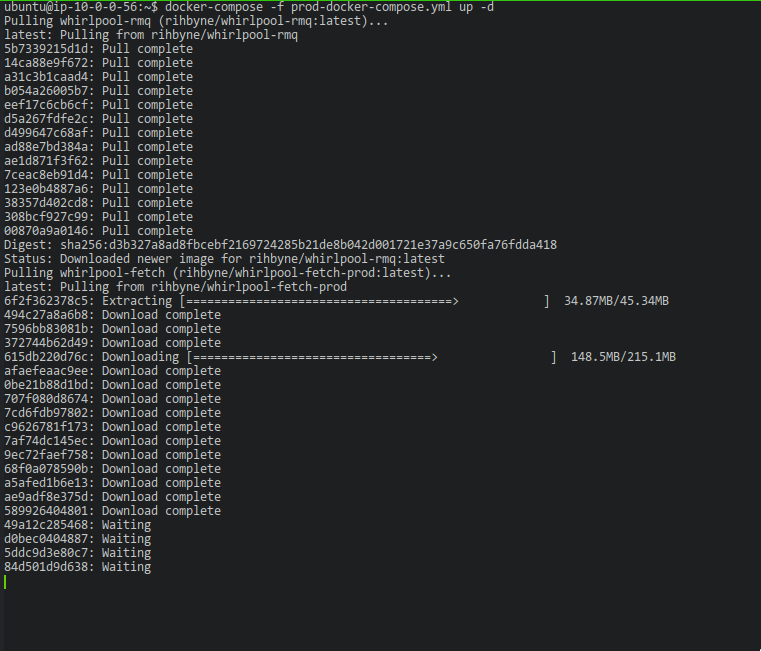
\includegraphics[width=15cm,height=15cm,keepaspectratio]{../media/crawler/docker-pull-prod.png}
  \caption{docker pull, extract, start containers}
  \label{fig:dockerpull}
\end{figure}

\noindent
Deleting the stack \texttt{whirlpool-crawler} terminates ec2 machines and dependent components in 
chronological order.

\begin{lstlisting}[language=bash]
  $ aws cloudformation delete-stack --stack-name whirlpool-crawler
\end{lstlisting}

\pagebreak